%%%%%%%%%%%%%%%%%%%%%%%%%%%%%%%%%%%%%%%%%
% Developer CV
% LaTeX Class
% Version 2.0 (21/05/2023)
%
% Authors:
% Will Fantom (willf@ntom.dev)
% Based on a template by Jan Küster (info@jankuester.com) and Jan Vorisek (jan@vorisek.me)
%
% License:
% The MIT License (see included LICENSE file)
%
%%%%%%%%%%%%%%%%%%%%%%%%%%%%%%%%%%%%%%%%%

%----------------------------------------------------------------
%	PACKAGES AND OTHER DOCUMENT CONFIGURATIONS
%----------------------------------------------------------------

\documentclass[9pt]{developercv} % Default font size, values from 8-12pt are recommended

%----------------------------------------------------------------

\begin{document}

%----------------------------------------------------------------
%	TITLE AND CONTACT INFORMATION
%----------------------------------------------------------------

\begin{minipage}[t]{0.38\textwidth} % 38% of the page width for name
	\vspace{-\baselineskip} % Required for vertically aligning minipages

	% If your name is very short, use just one of the lines below
	% If your name is very long, reduce the font size or make the minipage wider and reduce the others proportionately
	\colorbox{black}{{\HUGE\textcolor{white}{\textbf{\MakeUppercase{Will}}}}}\hspace{0.35cm}\footnotesize{(he/him)} % First name

	\colorbox{black}{{\HUGE\textcolor{white}{\textbf{\MakeUppercase{Fantom}}}}} % Last name

	\vspace{6pt}

	{\huge Researcher, Inventor,\\ Developer, Wizard, Nerd} % Career or current job title
\end{minipage}
\begin{minipage}[t]{0.22\textwidth} % 27.5% of the page width for the first row of icons
	\vspace{-\baselineskip} % Required for vertically aligning minipages

	% The first parameter is the FontAwesome icon name, the second is the box size and the third is the text
	% Other icons can be found by referring to fontawesome.pdf (supplied with the template) and using the word after \fa in the command for the icon you want
	\icon{MapMarker}{12}{lancaster, uk}\\
	\icon{Phone}{12}{+44 742 8147 463}\\
	\icon{At}{12}{\href{mailto:wf@ntom.dev}{wf@ntom.dev}}\\
\end{minipage}
\begin{minipage}[t]{0.22\textwidth} % 27.5% of the page width for the second row of icons
	\vspace{-\baselineskip} % Required for vertically aligning minipages
	\icon{Globe}{12}{\href{https://willfantom.dev}{willfantom.dev}}\\
	\icon{Github}{12}{\href{https://github.com/willfantom}{@willfantom}}\\
	\icon{Twitter}{12}{\href{https://twitter.com/@will\_fantom}{@will\_fantom}}\\
\end{minipage}
\begin{minipage}[t]{0.18\textwidth} % 18% of the page width for pic
	\vspace{-\baselineskip} % Required for vertically aligning minipages
	\hfill
	{%
		\setlength{\fboxsep}{0pt}%
		\setlength{\fboxrule}{5pt}%
		\fbox{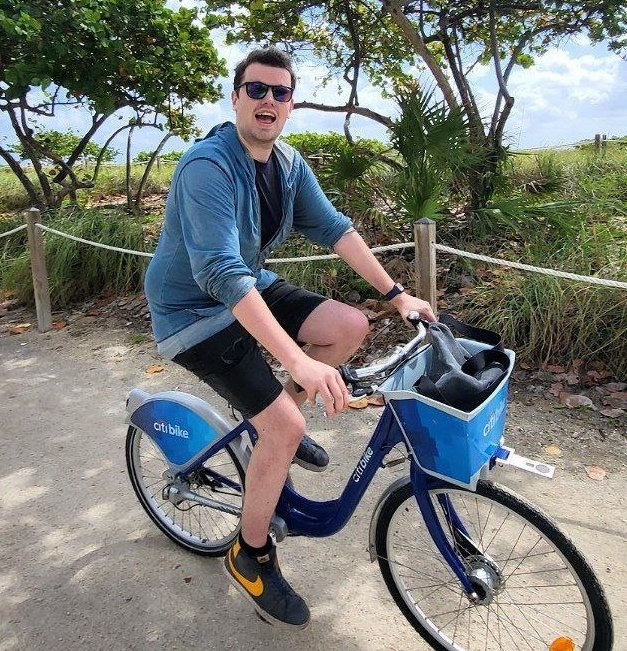
\includegraphics[width=0.8\linewidth]{assets/profile.jpg}}%
	}%
\end{minipage}

\vspace{0.15cm}

%----------------------------------------------------------------
%	INTRODUCTION, SKILLS AND TECHNOLOGIES
%----------------------------------------------------------------

\cvsect{Who Am I?}

\begin{minipage}[t]{0.35\textwidth} % 40% of the page width for the introduction text
	\vspace{-\baselineskip} % Required for vertically aligning minipages

	I am a systems researcher and PhD student with a focus on network and cloud
	infrastructures. The opportunities I have had to work alongside large tech
	companies in my research as they adopt modern software deployment workflows
	has allowed me to design and develop novel tools for cloud management and
	CI/CD. I typically spend my weekends on Pi projects and building apps for my
	home server.\\
\end{minipage}
\hfill % Whitespace between
\begin{minipage}[t]{0.31\textwidth} % 50% of the page for the skills bar chart
	\vspace{-\baselineskip} % Required for vertically aligning minipages
	\begin{barchart}{4.1}
		\baritem{Python}{82}
		\baritem{Go}{100}
		\baritem{C/C++}{68}
		\baritem{Java}{50}
		\baritem{LaTeX}{60}
		\baritem{Git}{80}
	\end{barchart}
\end{minipage}
\hfill % Whitespace between
\begin{minipage}[t]{0.29\textwidth} % 50% of the page for the skills bar chart
	\vspace{-\baselineskip}\vspace{-\baselineskip} % Required for vertically aligning minipages
	\cvsect{Tools}\\
	\mbox{\cvtag{Docker}\cvtag{LibVirt}\cvtag{Openstack}}
	\mbox{\cvtag{Kubernetes}\cvtag{FFMpeg}\cvtag{Linux}}
	\mbox{\cvtag{GitHub Actions}\cvtag{GitLab CI}}
	\mbox{\cvtag{DevContainer}\cvtag{Microsoft Word 2003}}
	\mbox{\cvtag{InfluxDB}\cvtag{OpenWRT}\cvtag{VS Code}}
\end{minipage}

%----------------------------------------------------------------
%	EXPERIENCE
%----------------------------------------------------------------

\vspace{-1em}
\cvsect{Experience}

\begin{entrylist}
	\entry
	{2023 -- Present}
	{Research Associate: AI4ME}
	{Lancaster University}
	{Working alongside the BBC and other academic partners to realize a testbed
		for multi-cloud deployments of object-based media applications. This focuses
		on how both micro and macroscopic telemetry can influence orchestration decisions.\\
		\texttt{Go}\slashsep\texttt{Docker}\slashsep\texttt{LibVirt}\slashsep\texttt{Consul}\slashsep\texttt{Cloud}\slashsep\texttt{Linux}}
	\entry
	{2019 -- 2022}
	{Associate Lecturer}
	{Lancaster University}
	{Designed, developed, implemented and taught a new novel software-defined
		networking coursework as part of the Advanced Networking undergraduate course.
		Also assisted in the delivery of the Distributed Systems course though lab
		assistance and mini Docker focused lectures.
		\\
		\texttt{OpenFlow \& SDN}\slashsep\texttt{Docker}\slashsep\texttt{Python}\slashsep\texttt{Java}\slashsep\texttt{Linux}}
	\entry
	{2020 -- 2022\\\footnotesize{part time}}
	{Research Associate: NG-CDI \& TOUCAN}
	{Lancaster University}
	{Worked alongside BT and other academic partners to investigate how cloud
		practices (primarily DevOps) could be utilized in network infrastructure as
		they transition from hardware-based deployments to software.\\
		\texttt{Go}\slashsep\texttt{C}\slashsep\texttt{GitHub Actions}\slashsep\texttt{Unikraft}\slashsep\texttt{Prometheus}\slashsep\texttt{Grafana}\slashsep\texttt{Træfik}}
\end{entrylist}

%----------------------------------------------------------------
%	EDUCATION
%----------------------------------------------------------------

\vspace{-1em}
\cvsect{Education}

\begin{entrylist}
	\entry
	{2018 -- present\\\footnotesize{ending approx. 2023}}
	{PhD -- Computer Science}
	{Lancaster University}
	{Working to integrate DevOps with network infrastructure operations through the
		development of novel CI/CD practices that support the strict requirements of
		low-level network functions and the emulation of context-specific hardware.}
	\entry
	{2015 -- 2018}
	{BSc (Hons) Computer Science \textit{(1st)}}
	{Lancaster University}
	{Thesis included the creation and evaluation of a custom x86 OS [fantomOS] that whilst
		monolitic, kept compile-time modularity in
		mind.\\\texttt{Operating Systems}\slashsep\texttt{Adv.
			Programming}\slashsep\texttt{Adv. Networking}\slashsep\texttt{Distributed Systems}\slashsep\texttt{...}}
\end{entrylist}

%----------------------------------------------------------------
%	PUBLICATIONS
%----------------------------------------------------------------

\vspace{-1em}
\cvsect{Publications}

\begin{entrylist}
	\pubentry
	{2023}
	{[1st Author]}
	{NES: Towards lifecycle automation for emulation-based experimentation}
	{IEEE/IFIP NOMS}
	\pubentry
	{2022}
	{}
	{Improving Intent Correctness with Automated Testing}
	{IEEE NetSoft}
	\pubentry
	{2022}
	{[1st Author]}
	{A NEAT way to test-driven network management}
	{IEEE/IFIP NOMS}
	\pubentry
	{2022}
	{}
	{Improving network resilience with Middlebox Minions}
	{IEEE/IFIP NOMS}
	\pubentry
	{2019}
	{}
	{DataPlane Broker: Open WAN control for multi-site service orchestration}
	{IEEE NFV/SDN}
\end{entrylist}

%----------------------------------------------------------------
% ADDITIONAL INFORMATION
%----------------------------------------------------------------

\begin{minipage}[t]{0.35\textwidth}
	\vspace{-\baselineskip} % Required for vertically aligning minipages
	\cvsect{Hobbies}\\
	\cvtag{Home Media Server}\cvtag{Cycling}\cvtag{Coffee}\cvtag{Dog
		Walks}\cvtag{Pi Dev Projects}\cvtag{Mario Kart}
	\divider\\
	\begin{minipage}[t]{0.25\textwidth}
		\vspace{-\baselineskip} % Required for vertically aligning minipages
		
\includegraphics[width=1\linewidth]{assets/websiteqr.png}
	\end{minipage}
	\hfill
	\begin{minipage}[t]{0.75\textwidth}
		\vspace{-\baselineskip} % Required for vertically aligning minipages
		Scan this QR Code to make sure you are seeing the latest version of my CV.\\
		Compiled on \textit{\today}\\
	\end{minipage}
\end{minipage}
\hfill
\begin{minipage}[t]{0.6\textwidth}
	\vspace{-\baselineskip} % Required for vertically aligning minipages
	\cvsect{Project: NES}\\
	Lead developer on a first of a kind cloud-native Network Emulation as a
	Service (NEaaS) platform we called NES. This system leverages various emulation
	technologies and unix networking tools to allow for the automated testing of
	large-scale virtual networks. Also included the development of layer 2 mesh
	network solution. All development work was done in Go and is packaged and
	deployed using Docker automatically via GitHub Actions. This is now used and
	developed in
	projects with partners such as BT and BBC.
\end{minipage}

%----------------------------------------------------------------

\end{document}
